\chapter{耳及颞骨}

\section{检查方法}

\subsection{常规检查}

1.横断面(轴位):为常用位置,扫描基线常用听眶上线(听眉线),扫描范围自外耳孔中心向上至岩锥上缘,共约15mm的范围。层厚、层距为1.0~1.5mm。一次扫描双侧,可再分别重建单侧图像,骨算法重建(HRCT)。以窗宽4000Hu左右,窗位400~800Hu摄取图像,重点显示软组织可用软组织窗观察。

2.冠状面:取仰卧或俯卧,扫描基线与听眦线大致垂直,自外耳孔前缘开始以1.5~2mm层厚向后扫描8~12层面。改良冠状位采用与枕骨斜坡平行层面为基线,骨算法重建(HRCT)。

3.直接矢状面扫描:很少应用。

\subsection{螺旋CT三维成像}

显示听小骨较佳,扫描层厚、层距1~1.5mm,重建层距0.1mm,能显示其立体形态,并能观察较小的骨质改变。多层面重组像可取代冠状、斜矢状面CT扫描。此外,中耳CT仿真内镜(CTVE)的应用有利于先天性中耳畸形、外伤后听骨链有无骨折脱位的观察,以及慢性中耳炎术前诊断、手术计划的制定和术后追踪观察。

\subsection{螺旋CT三维透明重建}

三维透明重建是对所选择的三维组织或物体内的所有像素进行投影,相当于模拟数字X线图像,可以观察内部结构,是一种透明法图像。目前,它已应用于胆囊、胃、结肠、输尿管、血管等空腔脏器。内耳又称迷路,外层骨质为骨迷路,其内有依附骨迷路分布的膜管和膜囊称为膜迷路,膜迷路内含有淋巴液。应用螺旋CT三维透明重建技术能清楚的显示膜迷路的精细结构及膜迷路囊、管间的相互关系,其图像立体直观。由于内耳结构排列方位不同,沿X轴和沿Y轴旋转的不同角度和不同位置对椭圆囊、球囊、前半规管、外半规管、后半规管、前庭窗、蜗窗、蜗管和内耳道等膜迷路结构的显示程度有明显差别。故应按具体要求选择适当的观察位置和角度以利于各结构的显示。同时,扫描时应注意尽可能的保证扫描基线的一致,使两侧耳部左右对称,以利于对比观察。

\section{正常解剖和CT表现}

\subsection{颞骨及耳部的解剖分部}

1.颞骨分为4部分:①鳞部:构成颅骨穹隆的外侧及部分外耳道。②乳突部:位于颞骨后部、锥体下方呈乳状突出,向下伸展构成乳突尖端。③岩部:又称岩锥或锥体,内耳及中耳的大部分和部分咽鼓管位于其中。由内耳孔向外伸展的长约10mm的骨性管道称为内耳道。④鼓部:呈半环状,构成外耳道的前壁及下壁。

2.耳部分为3部分:外耳、中耳、内耳。

\subsection{外耳}

外耳由耳廓和外耳道组成,耳廓为软骨。外耳道管径约1cm,长约2.5cm,外1/3为软骨段,内2/3为骨段,两者交界处称为峡部。软骨段和骨段CT均可显示。新生儿外耳道较短,全由软骨组成。成人由于骨膜呈倾斜状,故外耳道前下壁较后上壁长。骨段外耳道后上部由颞骨鳞部和岩部构成,前、下、后壁由鼓部组成,鼓部上部缺如。鼓沟为骨膜紧张部附着处。

鼓室盾板:又称骨膜嵴,为外耳道上壁内端与上鼓室外壁交界处的骨嵴,是上鼓室胆脂瘤常见破坏之处,在冠状面上显示最清楚(图\ref{fig4-1}-A、B)。鼓室盾板与锤骨之间的空隙称为普鲁萨克间隙(Prussak
pouch space),也是在冠状面显示最清楚,胆脂瘤常引起此间隙扩大。


\begin{figure}
  \centering
  \subfloat[正常颞骨冠状面]{
  \begin{minipage}[b]{0.5\textwidth}
    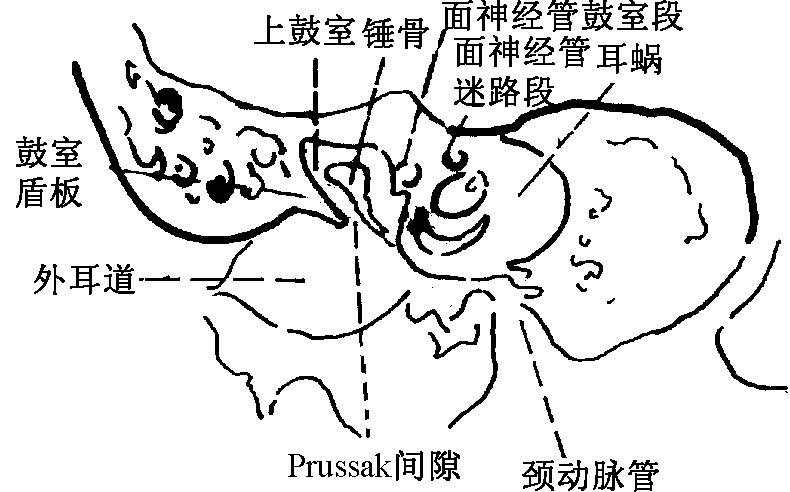
\includegraphics{./images/Image00108.jpg}\\
    {\small 右外耳道上缘内端骨嵴为鼓室盾板,与其内侧锤骨间有普鲁萨克间隙。右耳蜗外上缘双环影是面神经管前膝断面}
  \end{minipage}}\\
  \subfloat[正常颞骨冠状面]{
  \begin{minipage}[b]{0.5\textwidth}
    
\includegraphics{./images/Image00109.jpg}\\
    {\small 外耳道上壁内端向下突起为鼓室盾板,其内侧听小骨呈“L”状}
  \end{minipage}}\\
  \subfloat[正常颞骨冠状面]{
  \begin{minipage}[b]{0.5\textwidth}
    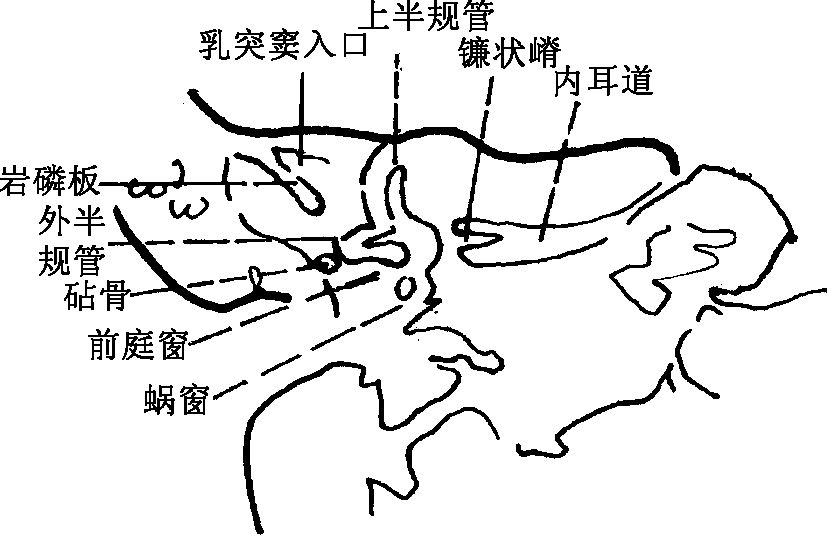
\includegraphics{./images/Image00110.jpg}\\
    {\small 骨迷路中央小圆形低密度影为前庭,前庭外侧管道为外半规管,外半规管下的前庭外壁缺口为前庭窗,外下壁缺口为蜗窗。骨迷路外含气腔为乳突窦入口,其中骨条影为岩鳞板}
  \end{minipage}}
  \caption{}
  \label{fig4-1}
  \end{figure}

  \begin{figure}
    \ContinuedFloat             %%<-- put this in subsequest figures.
    \centering
    \subfloat[正常颞骨冠状面]{
      \begin{minipage}[b]{0.5\textwidth}
        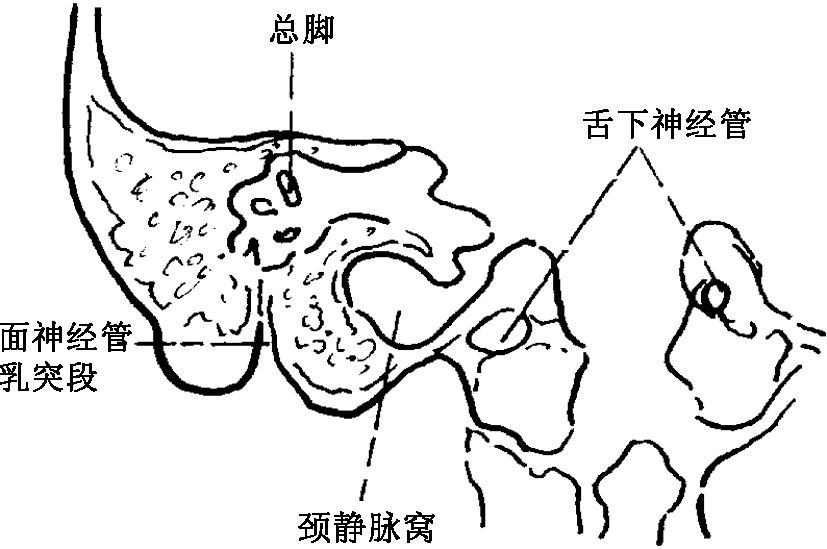
\includegraphics{./images/Image00111.jpg}\\
        {\small 骨迷路为总脚后层,其下方垂直管道为面神经管乳突段}
      \end{minipage}}\\
      \subfloat[正常颞骨横断面]{
      \begin{minipage}[b]{0.5\textwidth}
        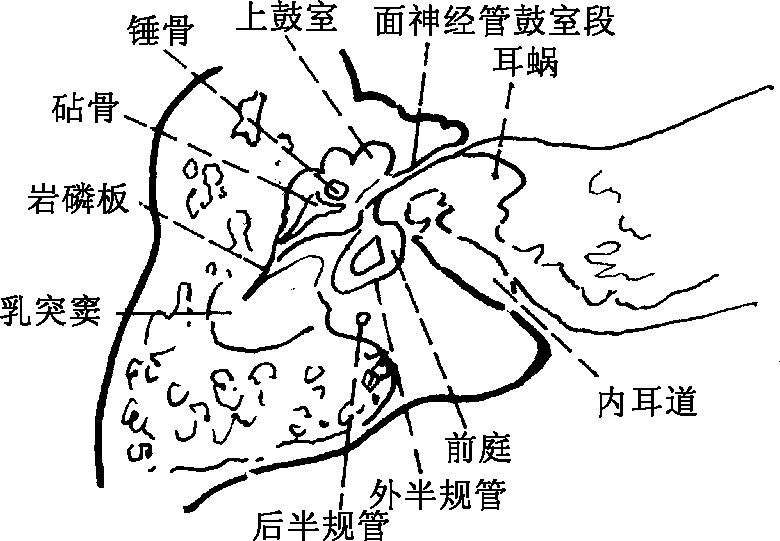
\includegraphics{./images/Image00112.jpg}\\
        {\small 在上鼓室的中央,锤骨与砧骨形如“冰淇淋蛋卷”。砧骨体内侧的长脚仅根部显示}
      \end{minipage}}\\
      \subfloat[正常颞骨横断面]{
      \begin{minipage}[b]{0.5\textwidth}
        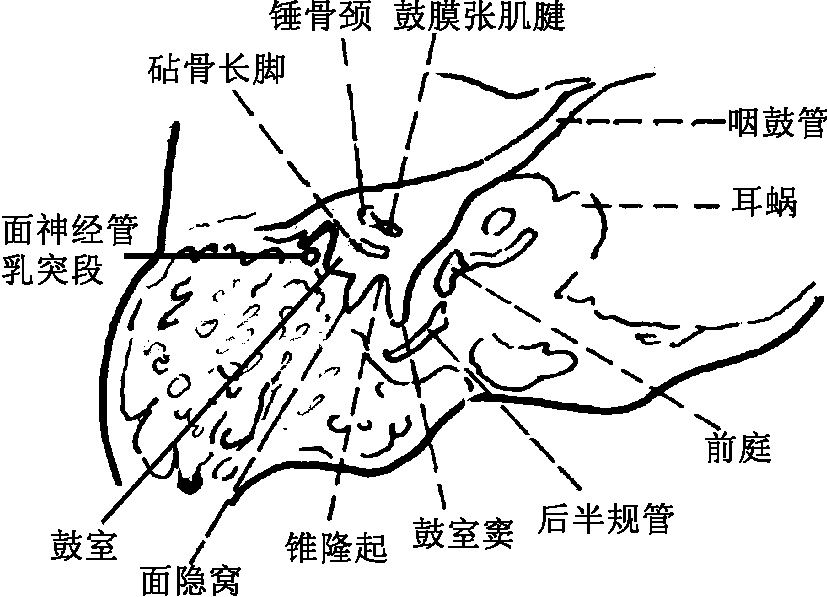
\includegraphics{./images/Image00113.jpg}\\
        {\small 骨迷路为耳蜗,其外含气腔为鼓室,鼓室后壁靠外的含气隐窝为面隐窝,靠内的隐窝为鼓室窦,面隐窝与鼓室窦之间的骨隆起为锥隆起}
      \end{minipage}}
      \caption[]{}
  \end{figure}

  \begin{figure}
    \ContinuedFloat             %%<-- put this in subsequest figures.
    \centering
    \subfloat[正常颞骨横断面]{
      \begin{minipage}[b]{0.5\textwidth}
        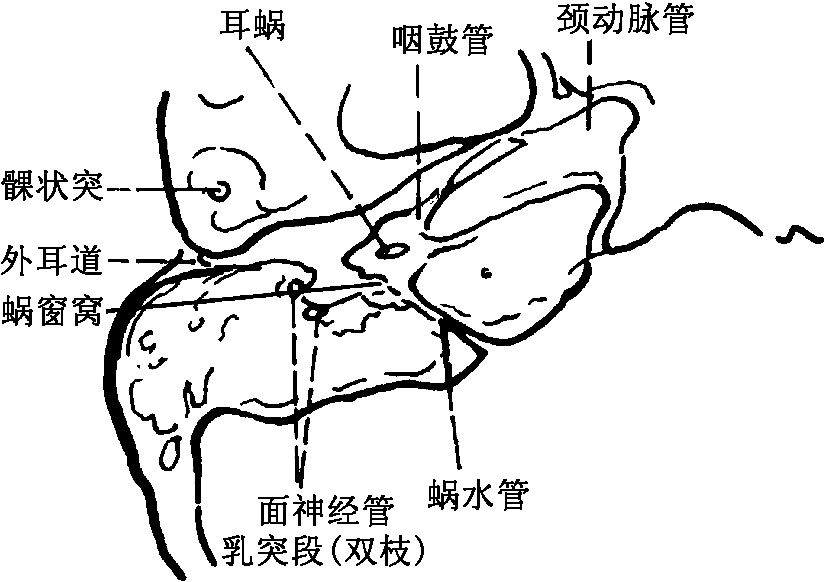
\includegraphics{./images/Image00114.jpg}\\
        {\small 右外耳道后壁与鼓室外壁交角处的厚壁小环影为面神经乳突段断面}
      \end{minipage}}\\
      \subfloat[正常颞骨横断面]{
      \begin{minipage}[b]{0.5\textwidth}
        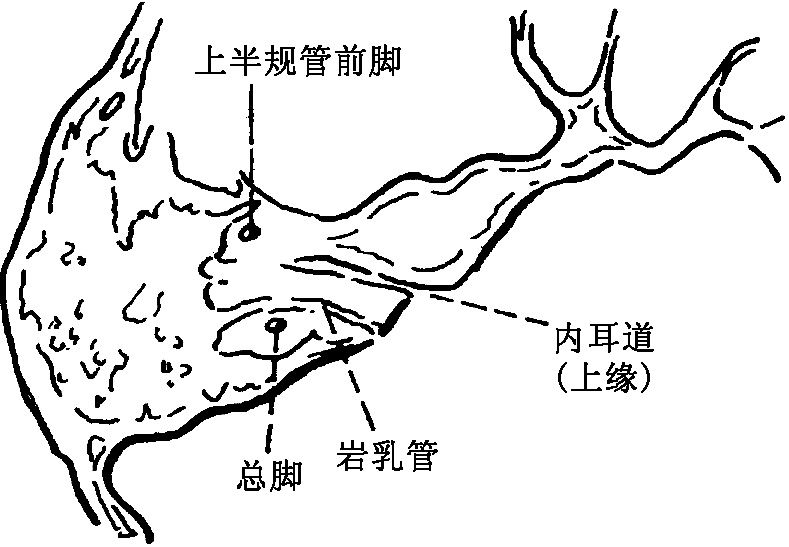
\includegraphics{./images/Image00115.jpg}\\
        {\small 岩部靠上的层面见双环影,前环为上半规管前脚,后环为总脚,两环之间的弧形细管道为岩乳管}
      \end{minipage}}\\
      \caption[]{}
  \end{figure}

\subsection{中耳}

1.鼓膜:为一层0.1mm厚的半透明、椭圆形薄膜。鼓膜上1/4为松弛部,下3/4为紧张部。鼓膜穿孔CT不能显示。鼓室是充满空气的空腔,以鼓膜为标志,其内侧为中鼓室,其上为上鼓室,其下为下鼓室。

2.鼓室:即中耳腔,向前经咽鼓管与鼻咽腔相通,向后经鼓窦入口及鼓窦与乳突气房相通。鼓室腔共有6个壁。①外侧壁:即鼓膜。②上壁(顶壁):又称鼓室盖壁,为一薄层骨板。③下壁(底壁):又称颈静脉壁,为一层向上凸起的薄骨板与颈内静脉上球分隔。此板可不完整或完全缺如,使颈内静脉完全疝入鼓室腔。④前壁:又称颈动脉壁,由颈内动脉垂直段后外壁组成。此壁有时不完整,为中耳炎症向前扩散的途径。⑤后壁:又称乳突壁,上部有鼓窦入口,开口的下方有一小的锥形骨隆起,称为锥隆起。蹬骨肌由锥隆起顶端发出,止于蹬骨颈的后侧。锥隆起外侧为面神经隐窝,隐窝的后内侧为面神经垂直段。锥隆起的内侧为鼓室窦(锥隐窝),它是前庭窗、蜗窗与鼓室后壁之间的空隙(图\ref{fig4-1}-F)。⑥内壁:又称迷路壁,即内耳骨迷路外侧壁,其中部稍膨出称骨岬(即耳蜗基底周)。骨岬后上方卵圆形的前庭窗(卵圆窗),由蹬骨底板和环韧带所封闭。骨岬后下方有圆形的蜗窗(圆窗),被蜗窗膜(第二骨膜)封闭。蜗窗位于前庭窗后1mm的下方,冠状面可见于前庭窗后1mm的层面,呈骨迷路外下缘的小缺口(图\ref{fig4-1}-C)。鼓室内有三块听小骨即锤骨、砧骨和蹬骨。

上鼓室在轴位像上呈底边在前的倒三角形,向后经乳突窦入口通向乳突窦。上鼓室在冠状面也呈三角形,底在上(即鼓室盖)与中颅窝相隔。正常值范围:左右径为6.79~6.97mm,前后径为9.58~9.84mm。

3.咽鼓管:沟通鼓室和咽腔。长3.5~4cm,鼓口比咽口高约2~2.5cm。

4.鼓窦:又称乳突窦,是鼓室后上方的一个含气腔,向前经鼓窦入口(宽约1~3mm)与上鼓室相通。成人鼓窦容量约1ml,上下径为1.5~7mm,平均为4.5mm;宽径为1~5mm,平均为2.5mm。其内壁为外半规管,顶壁为鼓室盖。

\subsection{听小骨}

听小骨的分布:听骨链位于鼓室内,锤骨柄附着在鼓膜上,锤骨头与砧骨体形成关节,位于上鼓室内形似“冰淇淋蛋卷”(图\ref{fig4-1}-E)。砧骨的长突与蹬骨形成关节,短突在轴位上指向鼓窦入口。听小骨中蹬骨最小,有前、后脚和蹬板,蹬板位于卵圆窗内。蹬板太薄CT不能显示,蹬骨脚可以显示。在冠状位上可显示砧骨长突与蹬骨形成的砧蹬关节。

轴位:连续扫描从低到高以1~1.5mm层厚和层距观察。第一层,中鼓室腔内高密度线状影为锤骨柄,其后偶尔见到砧骨长突远段。第二层,中鼓室腔内哑铃状结构,自外前向内后依次为锤骨颈、砧骨长突远段和蹬骨小头,后两者之间线状透亮区代表砧蹬关节。第三层,锤骨颈移行为锤骨头,位于鼓室前部,砧骨体和长突近段位于其后。第四层,锤骨头呈卵圆形位于上鼓室前部,其后方三角形结构为砧骨体和砧骨短突,锤砧关节清晰可见,宽约0.67mm±0.15mm(图\ref{fig4-1}-E)。

冠状位:连续扫描自前向后以1~1.5mm层厚和层距观察。第一层,锤骨头位于上鼓室偏外侧,锤骨颈和柄连于下方伸入到中鼓室。第二层,锤骨头和砧骨体沿鼓室外侧壁平行走行,中鼓室腔内锤骨柄清晰可见。第三层,上鼓室盾板内侧砧骨长突和蹬骨呈L状(图\ref{fig4-1}-B),两者连接处的透亮线为砧蹬关节。第四层,鼓室外侧壁和水平半规管间点状高密度为砧骨短突。(图\ref{fig4-1}-C)。

\subsection{内耳}

内耳又称迷路,埋藏在颞骨岩部,介于鼓室内壁与内耳道底部间,其长轴约2cm,与岩骨长轴一致。内耳外层的致密骨质称为骨迷路,其内相应分布的膜管和膜囊称膜迷路。两者之间隙充满外淋巴液,膜迷路内含有内淋巴液,两种淋巴系统互不相通。骨迷路可分为前庭、半规管和耳蜗3部分。

1.前庭:呈椭圆形腔室,最大横径应<3.7mm,位于耳蜗与半规管之间,其内容纳椭圆囊和球囊。其前下部较狭,与耳蜗的前庭阶相通;后上部相对较宽,有5个开口与骨半规管相接。前庭外壁为鼓室腔内壁,有前庭窗开口。前庭在横断面呈长椭圆形(图\ref{fig4-1}-E、F),冠状面呈类圆形含液腔(图\ref{fig4-1}-C)。

2.骨半规管:每侧有3条,分别称为外半规管(水平半规管)、上半规管(前垂直半规管)、后半规管(后垂直半规管),均位于前庭后方,三者相互垂直。每个半规管弯成2/3的环状,管径为0.8~1.0mm;各有两脚,一脚末端膨大叫壶腹,另一脚称单脚。上半规管和后半规管的单脚合为一总脚开口于前庭后部,其他各脚单独开口,故前庭后部有5个口与半规管相接。横断面显示外半规管较好(图\ref{fig4-1}-E),冠状面显示各半规管均佳(图\ref{fig4-1}-C、D
)。横断面上颞骨靠上层面可显示2个或3个半规管断面影;显示2个时,前环为上半规管前脚,后环为总脚(图\ref{fig4-1}-H);显示3个环时,前环及中环分别为上半规管前脚和总脚,后环为后半规管弓部断面。横断面上,总脚与上半规管前脚之间可见向前弯曲的细管道影为岩乳管,内含弓下动、静脉(图\ref{fig4-1}-H)。

3.耳蜗:位居前庭前部,形如蜗牛壳,从基底至顶部高约5mm。其蜗顶尖朝向前外方,接近咽鼓管鼓口;基底向后内方,长轴与岩锥后缘垂直。耳蜗中央为疏松骨构成的蜗轴,外绕以2.5~2.75周的螺旋骨管,分别称基底周、中周和尖周。基底周最宽,外侧凸出于鼓室腔内壁称骨岬,尖周最小。蜗顶上半部叫前庭阶,下半部叫鼓阶,两者在蜗顶部由蜗孔交通。耳蜗大致呈致密骨密度,边界清楚,与相邻颞骨结构有明显密度对比,易于辨认(图\ref{fig4-1}-F)。蜗轴为骨松质,CT不能清楚显示。

\subsection{耳蜗导水管及前庭导水管}

1.耳蜗导水管:为喇叭形的骨小管,成人全长6~10mm,宽约1mm,开口<6mm。起源于前庭阶底,向后内止于颅底颈静脉孔的外缘即岩锥下面颈静脉窝和颈动脉外口之间的三角形陷凹内,开口呈喇叭状。走行与内听道平行并位于其下方,横断面及冠状面可显示其开口(线图\ref{fig4-1}-G)。脑膜呈管状楔入此管,使蛛网膜下腔和内外淋巴间隙沟通。此导水管有调节脑脊液和外淋巴液间压力的功能,故也是脑膜炎播散至内耳迷路的通道。该管腔扩大至正常的2倍以上时有临床诊断价值。

2.前庭导水管:包括内淋巴管和内淋巴囊两部分,位于岩锥内。内淋巴管起始于椭圆囊管和球囊管交界处,在前庭的后上、半规管总脚附近穿出,与后半规管走行方向一致,呈30°~60°角向后下开口于岩锥内后缘、后半规管内侧、内耳孔后下方一骨浅窝内的内淋巴囊。该淋巴囊位于两层脑膜之间,内淋巴囊在CT上无法显示。前庭导水管管径远较蜗导水管细小,中份内腔横径<1.5mm,前庭导水管开口在横断面CT图像上有时可以显示。

\subsection{内耳道}

又称内听道,正常形态多呈管状,亦可略呈壶腹状或喇叭状。两侧大致对称,长约10mm。正常内听道上下径为4~7.5mm,平均5.9mm;前后径为4~7mm,平均为5.7mm;30%正常人两侧之宽度可有1~2mm的差别。内耳道靠底部有横行骨嵴为镰状嵴,冠状面呈横行致密线,为内耳道的标志(图\ref{fig4-1}-C)。镰状嵴将内耳道分成上下两部分。①上部:较小,前方为面神经区;后方呈漏斗状为前庭上区,听神经的前庭上神经由此进入,终止于椭圆囊和上、外半规管。②下部:较大,前方为蜗区,是听神经的蜗支进入耳蜗的通道;后方为前庭下区,有听神经的前庭下神经通过,终止于球囊。

\subsection{颈静脉孔}

1.颈动脉管:位于颞骨岩锥内,冠状面位于耳蜗之下,横断面于岩骨尖可见沿颞骨外缘向内前走行的带状管道(图\ref{fig4-1}-A、G)。

2.颈静脉孔(或颈静脉窝):位于颞骨岩部与枕骨之间岩枕裂内,呈葫芦样。颈静脉窝位于中耳鼓室的下方,两者之间有骨性间隔。颈静脉孔(窝)中间有一骨棘将其分为两部分。①神经部:较小,位于前内,主要含舌咽神经。②血管部:较大,位于后外,主要含颈静脉球、迷走神经及副神经等。右侧一般大于左侧,原因是右侧颈静脉和乙状窦较大。

有报道颈静脉孔(窝)血管部横径平均为10mm,神经部横径平均为9mm,其总长径平均为15mm。根据测量指标难以判断正常或异常,主要根据其他征象如骨质情况及增强表现予以判断。颈静脉窝横断面及冠状面均可见(图\ref{fig4-1}-D),两侧多不对称。正常窝顶不超过蜗窗水平,超过此水平未必有症状,但应提示高位。正常颈静脉窝与鼓室之间之骨性间隔缺损可为正常变异(称为高位颈静脉球或颈静脉球裸露)。

\subsection{面神经管}

面神经分为6段:①颅内段(又称脑池段);②内耳道段;③迷路段;④鼓室段(又称水平段);⑤垂直段(又称乳突段);⑥腮腺段(又称颅外段)。还有学者分为7段,即将下述的前膝作为一段。

面神经管可分为以下3段:

1.迷路段:横断面显示此段,沿耳蜗外上缘前外走行的低密度管道。面神经自内耳道底镰状嵴之上、向前内出内耳道,进入颞骨岩部面神经管的迷路段,迷路段又分为近支和远支(图\ref{fig4-2})。近支起自内耳道底,向上向外,通过岩骨尖,走行于耳蜗和前庭之间,终止于膝状神经节窝,在此处面神经管呈锐角(75°)向后折返移行为远支,形成一倒“V”字形,这是第一次反折或称前膝。在冠状面上靠耳蜗外上缘可见两个小环影,靠内的小环为迷路段断面,靠外的小环为鼓室段起始部。如层面恰在神经管膝时则两环影相连。

\begin{figure}[!htbp]
 \centering
 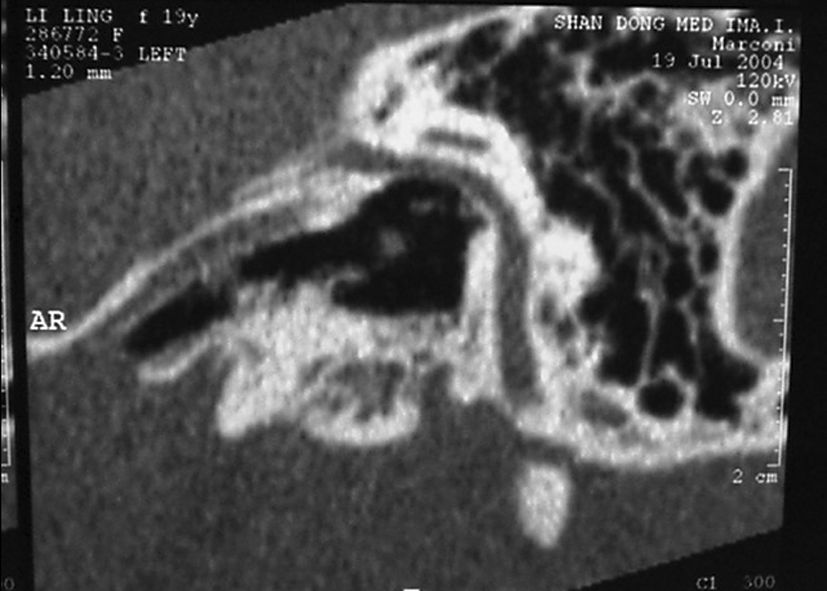
\includegraphics[width=.7\textwidth,height=\textheight,keepaspectratio]{./images/Image00116.jpg}
 \captionsetup{justification=centering}
 \caption{面神经管迷路段\\{\small 面神经管斜矢状面重建,呈由前上向外后走行的低密度管道}}
 \label{fig4-2}
  \end{figure} 

2.鼓室段(或称水平段):沿鼓室内壁上缘向后外走行,经前庭窗之上达于外半规管前脚下缘。横断面可见鼓室内壁前后走行的细管道(图\ref{fig4-1}-E)。冠状面于外半规管前角层面可见其下缘之面神经管切迹。面神经管鼓室段管壁的骨质部分缺损为常见的正常变异,CT难以显示。

3.垂直段(或称乳突段):面神经管出鼓室后向下屈曲95°~125°形成第二反折或称为后膝。沿鼓室后外壁下行于乳突部即垂直段。最后经茎乳孔出颅进入腮腺。冠状面上该段在后半规管或外半规管后脚之下,下行达茎突孔,茎突孔呈喇叭口状。横断面上该段在面神经隐窝外后及外耳道后壁内端之后,断面呈厚壁的环状,与附近薄壁的乳突蜂房有别。

\section{先天畸形和变异}

\subsection{中耳畸形}

外、中耳胚胎原基相同,而与内耳原基不同,外中耳来源于第一、第二对腮弓和第一腮裂、第一咽囊,故常常外耳和中耳都有畸形,但也有少数外、中、内耳均有畸形。中耳畸形主要有鼓室倾斜、狭窄及听骨链畸形。

\subsubsection{外耳道狭窄与闭锁}

为最常见的外、中耳畸形。CT多可显示,多同时伴有中耳畸形(图\ref{fig4-3})。国内有报道骨性外耳道的发育畸形(包括下述的垂直外耳道)大部分为颞骨鼓部未发育或发育不良所致。





\begin{figure}[!htbp]
 \centering
 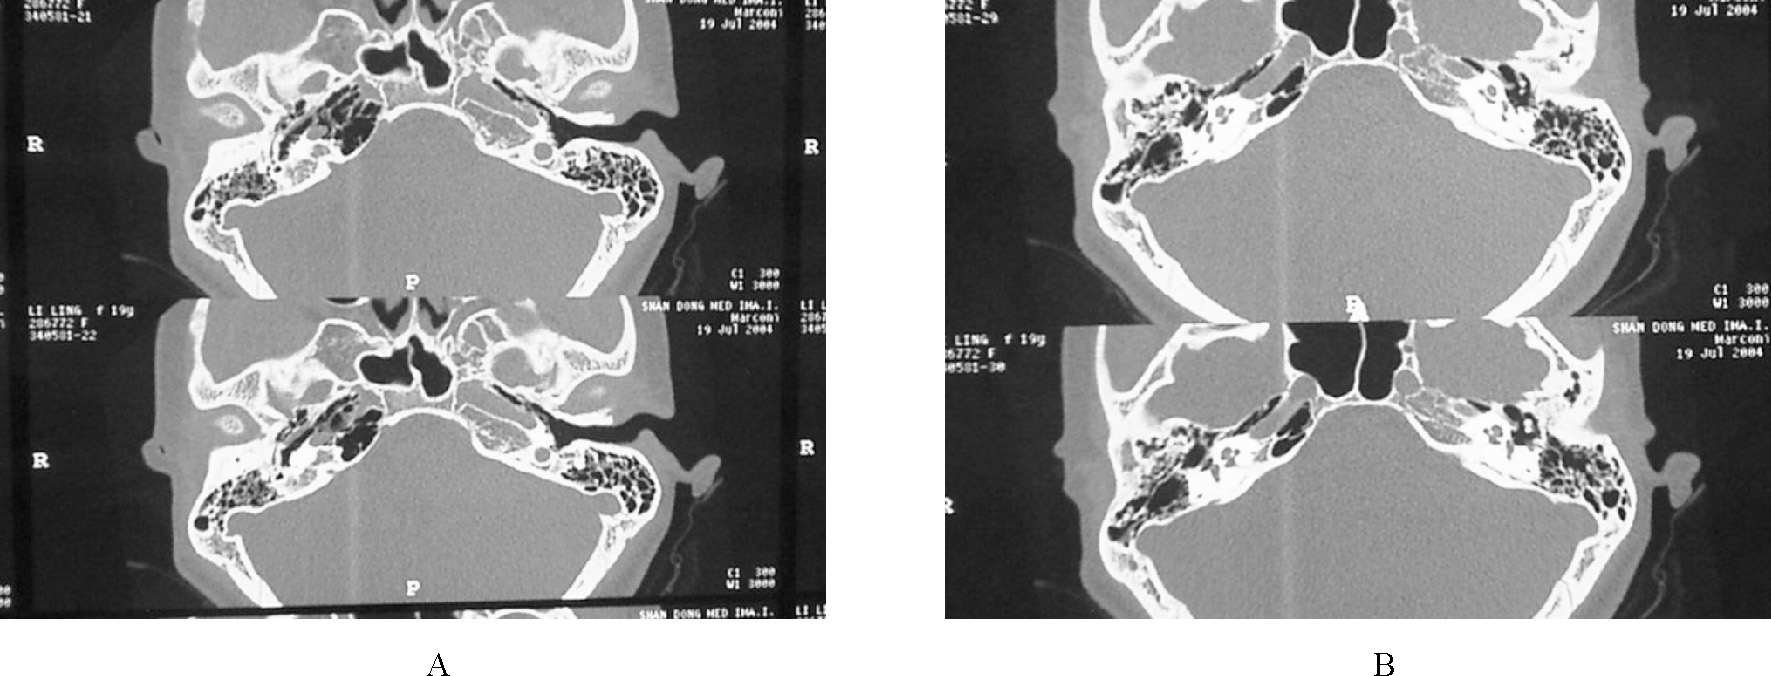
\includegraphics[width=.7\textwidth,height=\textheight,keepaspectratio]{./images/Image00117.jpg}
 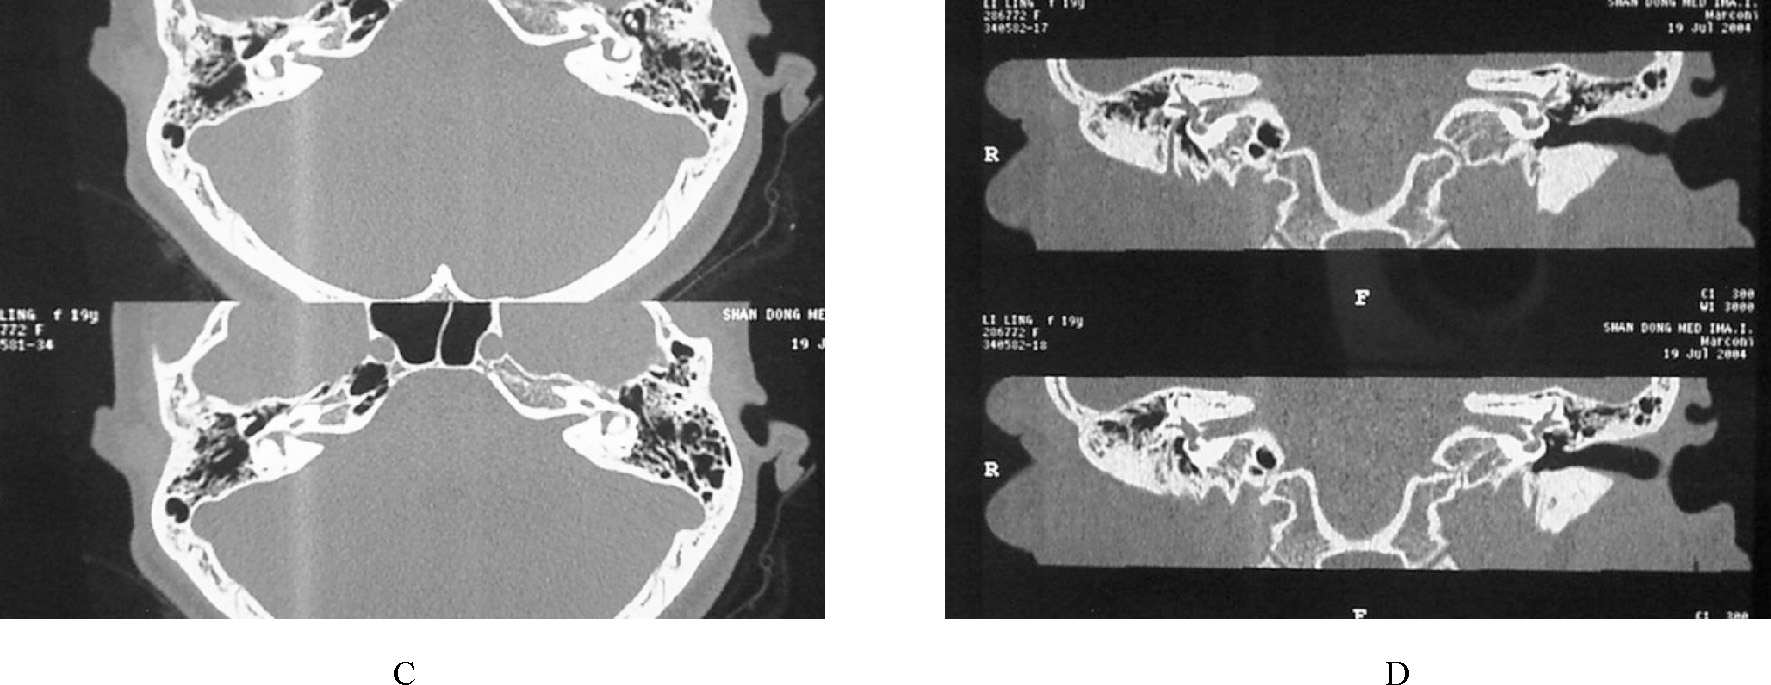
\includegraphics[width=.7\textwidth,height=\textheight,keepaspectratio]{./images/Image00118.jpg}
 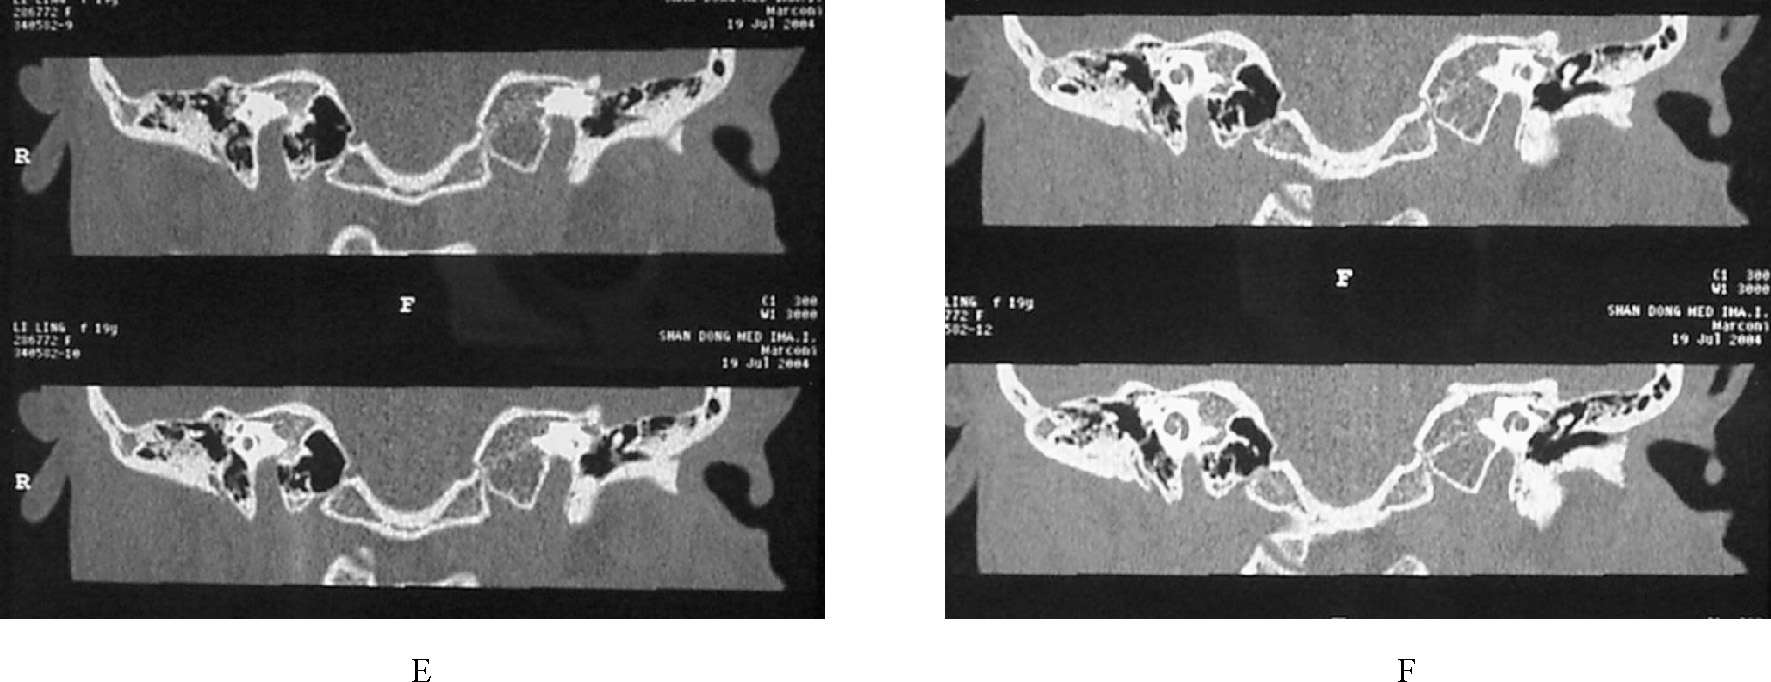
\includegraphics[width=.7\textwidth,height=\textheight,keepaspectratio]{./images/Image00119.jpg}
 \captionsetup{justification=centering}
 \caption{右侧外耳道闭锁并右侧听骨链发育异常}
 \label{fig4-3}
  \end{figure} 

CT表现为耳廓小于正常,呈条索状突起或残缺。外耳道狭窄与闭锁按部位可发生在骨部或软骨部,也出现可整个外耳道闭锁。按性质可分为骨性和膜性闭锁,前者无外耳道,代之以厚度不一的骨性闭锁板;后者外耳道为软组织密度影充填并与外耳道皮肤相连,骨性外耳道存在,但严重狭窄。外耳道狭窄是指外耳道前后径或上下径<4mm。

\subsubsection{垂直外耳道}

相当于正常外耳道部无外耳道结构,外耳道呈闭锁状。而自鼓室有骨性管道下行达颞骨下缘,管道内多充填软组织,亦可含气。

\subsubsection{听小骨畸形}

可单独发生,为最轻的外中耳畸形。先天性听骨链畸形以蹬骨畸形最多见,砧骨次之,前庭窗和蹬骨肌畸形并列第三位。锤砧畸形CT基本可显示,如锤砧关节融合、砧骨长脚缺如、锤砧骨变形增粗、锤砧关节交角异常等。虽然单纯蹬骨畸形多见,但CT难以显示。CTVE对上述畸形显示较好,但对听骨链的细微结构显示欠佳。此外,鼓室可发育小(多以下鼓室为著)甚至不发育(缺如),部分可伴同侧乳突气化不良或完全不气化。

\subsubsection{面神经管异常}

常见于外耳道闭锁患者,最常见有面神经管乳突段前位、鼓室段低位。

\subsection{内耳畸形}

内耳原基为神经外胚层衍生的听板及以后的听囊。内耳膜迷路来自外胚层,骨迷路来自中胚层。内耳畸形包括由听囊衍生的前庭、半规管、耳蜗、内淋巴囊、前庭导水管以及非听囊原因的内耳道畸形。CT只能显示骨质异常,MR可显示迷路影像。内耳畸形可导致先天性感音性耳聋。

\subsubsection{耳蜗畸形}

可见以下几种:①耳蜗缺如:无耳蜗形态,属米歇尔畸形(Michel
teratism,即内耳完全不发育,只有外耳和中耳)。②耳蜗与前庭共腔:无内在结构,共腔可呈圆形或小提琴状。③耳蜗大小正常:但其间隔不全或缺如,呈空窝状。④耳蜗发育小及形状异常:即耳蜗的圈数减少不及2周,尖部和中间圈连合成为一单腔,应属蒙迪尼畸形(Mondini
teratism)。⑤Mondini-Alexander畸形:除有耳蜗畸形外,还有前庭的畸形。

\subsubsection{前庭畸形}

常见的是前庭腔扩大。正常前庭横径<3.7mm,如>3.7mm且临床上有先天性感音性耳聋即为前庭扩大畸形,耳蜗可无异常。如其他内耳结构均完全缺如则属米歇尔畸形。如内耳道底骨质完全缺损,则前庭与内耳道相通,脑脊液进入前庭,并可通过前庭窗蹬骨底板缺损进入鼓室,再通过咽鼓管进入鼻咽腔,形成脑脊液鼻漏,而出现相应的临床及CT表现。

\subsubsection{前庭导水管扩大}

属前庭导水管综合征。本病包括前庭导水管、内淋巴管和内淋巴囊扩大。

以下CT特点及临床资料可作为本病的诊断依据:①水平半规管或总脚层面显示岩锥后缘有深大三角形或裂隙状、边缘清晰的明显骨缺损影;②骨缺损影内端(即前庭导水管近段)与前庭或总脚直接相通;③前庭导水管中段的前后径>1.5mm,且边缘清晰;④临床有先天性感音性耳聋。

CT征象中尤以①和②最为重要(其中“边缘清晰”这一特点最为重要)。此外,本病常伴有内淋巴囊扩大,此亦为导致内淋巴囊裂扩大,形成岩锥后缘宽大骨缺损的原因之一。但同时有学者认为,不应将实为内淋巴囊裂的前庭导水管外口宽度>1.5mm(亦有人主张为\textgreater{}2.0mm)作为轴位诊断前庭导水管扩大的标准。

值得注意的是多数先天性内耳畸形可伴有或单独存在前庭导水管扩大畸形。

\subsubsection{半规管发育不良}

常见外半规管短小。前庭扩大畸形常伴各半规管发育不良,尤其多见外半规管短小或缺如。后半规管缺如为瓦登伯格(Waardenburg)综合征的影像特征。

\subsubsection{内耳道畸形}

内耳道宽度<3mm 需考虑为狭窄,此时听神经和(或)面神经发育不良。

\subsubsection{Scheibe畸形}

本病指仅有膜迷路的畸形,如骨迷路正常,故CT不能诊断。

\subsection{高位颈静脉球和颈动脉异位}

\subsubsection{高位颈静脉球}

亦称为颈静脉球裸露,是一种先天变异,为颈静脉窝与中耳腔之间的骨性分隔缺如,也可以有搏动性耳鸣等症状。动态CT增强扫描可进一步确诊。

\subsubsection{颈动脉异位}

亦称为迷走颈内动脉,是一种罕见的解剖变异。在正常颈动脉的位置以外,原始的血管持续存在,可造成颈内动脉位于中耳内,突入鼓室、达鼓岬外侧,是耳鸣的原因之一,多单独发生。

\section{外伤}

\subsection{概述}

颞骨外伤最多见为骨折,常见症状是耳出血、耳漏、耳聋和面瘫。

根据症状应注意观察的部位有:①耳出血及传音聋:应以外耳道、乳突、鼓室、听小骨为重点;②面瘫:以面神经管各段为重点;③感音聋:以骨迷路、内耳道为重点;④脑脊液耳漏:以鼓室盖、前庭、内耳道底为重点。

\subsection{颞骨骨折的分类}

分类:根据骨折线方向与锥体长轴的关系可分为两种类型:纵行骨折和横行骨折。但有的可兼有两种类型,有的呈斜行。①纵行骨折:一般从鳞部开始,向前向下,通过鼓室盖、外耳道、中耳和破裂孔。骨折可引起气脑、脑脊液漏,也可引起听小骨脱位和骨折。②横行骨折:不如纵行骨折常见,但较严重,常损伤骨迷路,向外可以损伤中耳。临床表现眩晕、神经性耳聋和面神经麻痹,并可有脑脊液漏。上述骨折冠状位及轴位均可显示,圆窗及卵圆窗部位的微小骨折CT不能显示。

有些正常结构不可误为骨折。正常结构有两侧对称的特点,如横断面的面神经管的迷路段和鼓室段,横断面的岩乳管,冠状面的岩鳞裂等。

\subsection{外伤性听骨链异常}

国内有学者统计外伤性听骨链异常以HRCT为优,其结果如下:①听骨链完全断裂,占30.3%;②锤砧关节脱位或伴有锤、砧骨移位,占48.5%;③锤砧骨移位,占12.1%;④砧蹬关节脱位,占6.1%;⑤蹬骨脚骨折,占3.0%。听鼓链最常见的损伤部位有砧骨、砧蹬关节相邻的部位以及砧蹬关节,锤砧关节脱位最常见。

锤砧关节脱位常意味着锤骨或砧骨不同程度的移位,两者可以单独移位或共同移位。以此判断是否移位或者脱位,要注意以下两个方面:①结合横、冠状面仔细观察,必要时利用矢状面;②双侧对照,扫描层厚尽量要薄,并且对称。听小骨骨折较脱位少见,骨折最常见的部位是蹬骨脚、砧骨长脚和锤骨颈,但不易诊断;特别是蹬骨结构细微,HRCT不易显示,骨折线难以观察。同样,对于砧蹬关节是否脱位常根据砧骨是否移位的间接征象来确定。

\section{炎症性疾病}

\subsection{坏死性外耳道炎}

本病又称恶性外耳道炎,是由绿脓杆菌所致的外耳道急性骨髓炎。

\textbf{【病理】}
外耳道肉芽组织、纤维组织增生及骨质破坏,常累及中耳。根据有无骨质破坏可分为早期和晚期两个阶段。早期只有软组织改变而无骨质破坏;晚期感染蔓延并有骨质破坏,可影响面神经和(或)其他颅神经、颞颌关节,出现相应症状和体征。

\textbf{【临床表现】}
常见于老年人及糖尿病患者。主要表现为疼痛、外耳道溢液、听力障碍以及外耳道肉芽肿,亦可出现面瘫、张口困难等。

\textbf{【CT表现】}
外耳道及中耳充以软组织,外耳道壁侵蚀性骨质破坏,可累及鼓室壁、颞颌关节、乳突、面神经管甚至岩部。鼻咽部及颞下窝软组织可肿胀。

本病CT表现无特异性,诊断需参考临床,与恶性肿瘤鉴别也要结合临床及活检。

\subsection{分泌性和气压损伤性中耳乳突炎}

中耳炎的分类:①按病原体分为化脓性和非化脓性;②按病程分为急性和慢性;③按病理分为分泌性(又称渗出性、浆液性、黏液性和卡他性)和化脓性。

\textbf{【病理】}
渗出性中耳炎为非感染性炎症,继发于咽鼓管阻塞。由于中耳腔和乳突气房内的气体被吸收后呈负压状态,导致黏膜血管舒张产生血清渗出、黏膜充血肿胀、咽鼓管黏液腺分泌增加。气压损伤性中耳炎与其病理改变一致,且气压损伤性中耳乳突炎与大气压急剧变化有关。但渗出性及气压损伤性中耳乳突炎均可由急性转为慢性。

\textbf{【临床表现】} 主要有耳聋、耳闷,耳痛、耳鸣,听力减退等症状。

\textbf{【CT表现】}
中耳及乳突气房消失,呈液体或软组织样密度,无骨质破坏。慢性者表现为气房骨壁骨质密度增高。

\textbf{【鉴别诊断】}
急性和慢性单纯型化脓性中耳乳突炎与分泌性中耳乳突炎病理上均为渗出改变,影像学表现也相近,区别仅为有无细菌感染,需要结合临床才能明确诊断和鉴别。

\subsection{急性化脓性中耳乳突炎}

本病是中耳黏膜的急性化脓性炎症。

\textbf{【病因病理】}
化脓性细菌多由咽鼓管侵入鼓室,病变常涉及鼓室、咽鼓管和乳突,也可经鼓膜途径(外伤、穿刺等)、血行感染(极少见)致病。致病菌主要为肺炎链球菌、流感嗜血杆菌、葡萄球菌等。初期病理表现为黏膜充血肿胀、炎性细胞浸润、炎性渗出物增加。继续发展炎性渗出物变为脓性,脓液积聚、鼓室内压力增高,可导致黏膜坏死、鼓膜穿孔。如治疗不当或有骨质坏死,病变迁延为慢性。

\textbf{【临床表现】}
好发于儿童,主要表现为耳痛,听力减退及耳鸣,鼓膜穿孔,耳溢液初为血水样、后为黏液脓性。如合并乳突炎则乳突部红肿、乳突尖有明显压痛。此外,尚有发热、头痛等全身症状。本病临床一般可做出诊断,CT主要了解骨质破坏程度和颅内并发症情况。

\textbf{【CT表现】}
乳突气房密度增高,气房间隔骨质吸收、密度减低。鼓室、乳突窦内积脓,表现为密度增高,有时可见液平。后颅窝薄层CT增强扫描可显示颅内并发症。

\subsection{慢性化脓性中耳乳突炎}

本病是由急性化脓性中耳乳突炎未经治疗或治疗不当发展而来,或因鼻咽部及邻近器官的慢性炎性病灶经咽鼓管感染所致。一般认为急性炎症超过2个月未愈即为慢性。少数无急性感染病史者,可由低毒力感染所致。

\textbf{【病理】}
可分为单纯型、肉芽肿型和胆脂瘤型3类。慢性化脓性中耳炎主要病理过程为渗出与肉芽组织形成,故胆脂瘤往往合并肉芽组织增生。①单纯型:又称黏膜型,黏膜充血肿胀、炎性细胞浸润,可有纤维组织增生和粘连。②肉芽肿型:又称坏死型、骨疡型,除上述单纯型的改变外,还有黏膜鳞状上皮化,肉芽组织增生或息肉形成,听小骨和上鼓室骨质有破坏。③胆脂瘤型:并非真性肿瘤。外耳道、鼓膜的上皮经鼓膜穿孔处移行长入鼓室,然后脱落堆积成团即形成胆脂瘤。其主要成分为脱落的角化上皮,可含有胆固醇。

\textbf{【临床表现】}
耳流脓史长达数年甚至数十年,有听力减退、耳鸣、眩晕、头痛等症状。体检见鼓膜紧张部穿孔并有脓液、肉芽组织或胆脂瘤上皮。听力检查多为传导性耳聋。

\textbf{【CT表现】}
能显示耳部的微细骨质变化,亦能显示软组织、积液,但胆脂瘤、胆固醇肉芽肿及炎性肉芽肿均表现为类似的软组织影,CT难以鉴别。

1.单纯型:鼓室黏膜增厚。气化好的乳突可见气房密度增高,无明显骨质破坏。硬化型乳突显示鼓窦周围骨质硬化(图\ref{fig4-4}A)。

2.肉芽肿型:①软组织形态呈不规则片网状、条索状,弥散分布(图\ref{fig4-4}B、C),增强扫描因肉芽组织富血管而强化;②听骨破坏少见,局限性侵犯,程度轻;③骨壁破坏偶见于鼓窦及入口,边缘模糊;④面神经管及鼓室盖破坏少见。

3.胆脂瘤型:①软组织形态呈团块状,CT值多为30~50Hu,亦可呈负值,边缘可见低密度圈;增强扫描无强化,但其周围炎性肉芽组织可形成强化环;②听骨破坏多见,程度较重;③骨壁破坏,边缘致密硬化、光滑是诊断的关键,可呈分叶状(图\ref{fig4-4}D);鼓窦、鼓室及鼓室入口扩大,盾板短钝;外耳道胆脂瘤可有外耳道膨大表现;④面神经管及鼓室盖破坏多见。

\begin{figure}[!htbp]
 \centering
 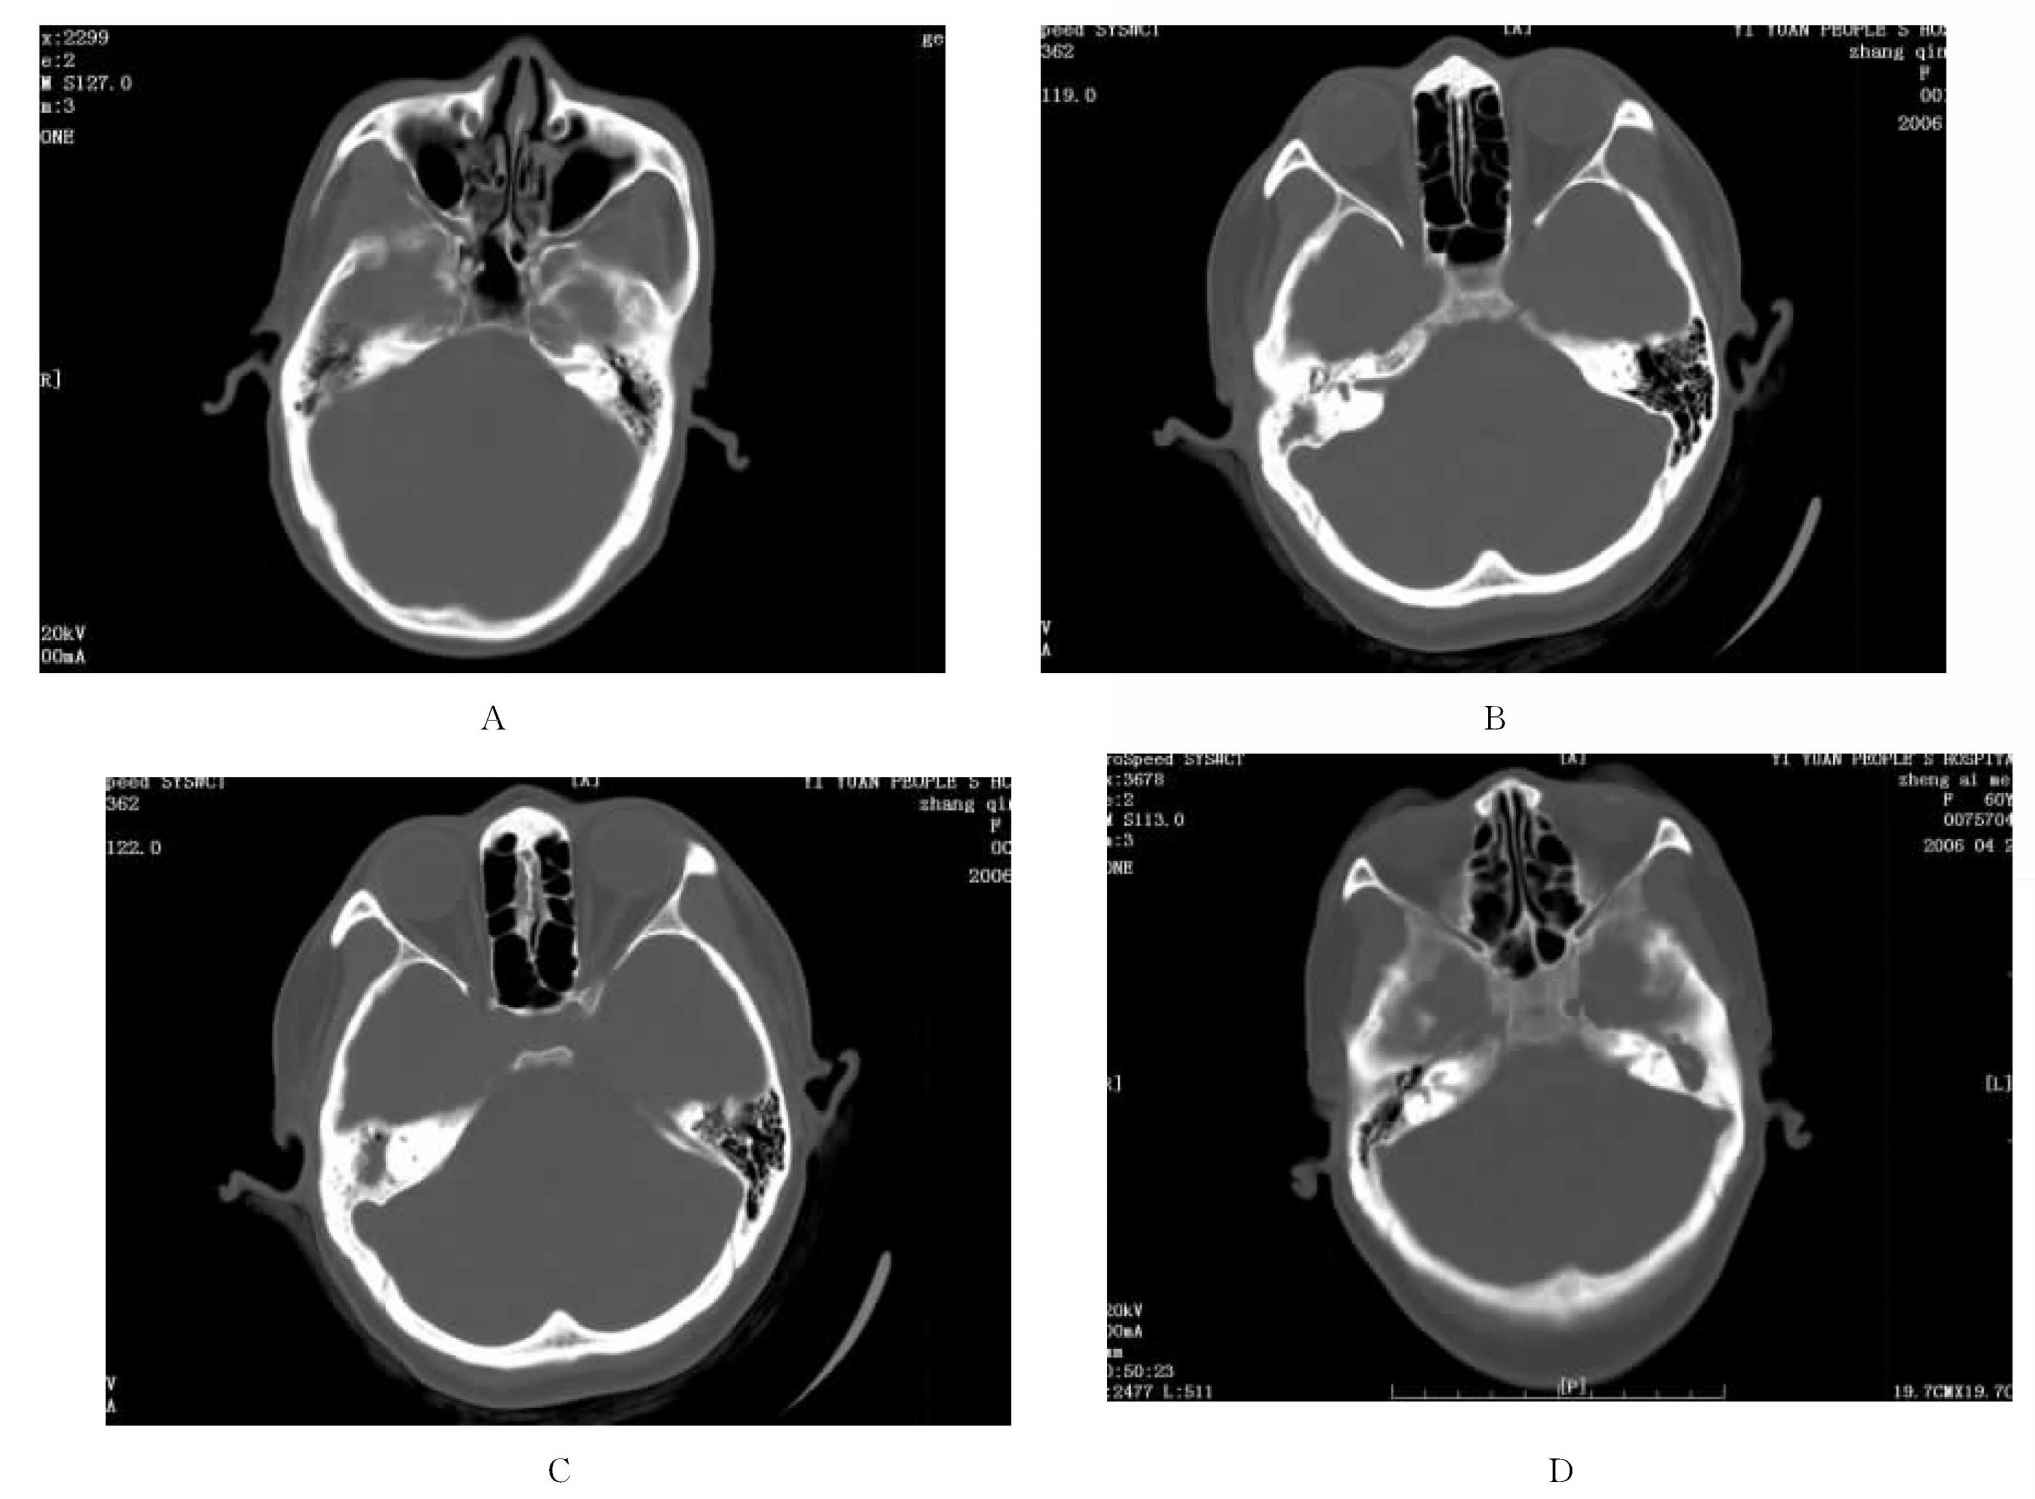
\includegraphics[width=.7\textwidth,height=\textheight,keepaspectratio]{./images/Image00120.jpg}
 \captionsetup{justification=centering}
 \caption{慢性化脓性中耳乳突炎\\{\small A.右侧Ⅰ型;B.右侧Ⅱ型,并显示右侧锤砧关节;C.右侧Ⅱ型;D.左侧Ⅲ型,右侧可见正常锤砧关节}}
 \label{fig4-4}
  \end{figure} 

此外,诊断时应注意以下两点。①鼓窦大小约6mm×10mm。当发生单纯型慢性中耳乳突炎时,鼓窦周围硬化,尤其由于长期慢性炎症使乳突呈硬化型的患者,可将正常鼓窦误为胆脂瘤,故对<10mm的低密度区诊断应予慎重。即使手术证实该腔内有胆脂瘤上皮,如无明显的膨大压迫征象,亦不应轻易诊断为胆脂瘤。因为有些患者鼓窦区虽有肉芽组织及胆脂瘤上皮存在,但并未形成具有被囊的胆脂瘤,而呈边缘不清的低密度区,即为肉芽肿型慢性中耳乳突炎。当然,胆脂瘤继发感染边缘亦可模糊,但仍有明显的膨大压迫表现有助于诊断。②一般认为慢性中耳炎患者硬化型乳突如无骨质破坏,以不称为慢性乳突炎为妥。因为硬化型乳突有多种因素(如幼年期发生中耳炎、遗传等)所致发育障碍的结果,并非乳突本身有活动性炎症。即使长期慢性化脓性中耳炎可引起骨质硬化,形成硬化性乳突,但硬化型或板障型乳突对炎症的扩展有一定阻碍,如无骨质破坏,炎症一般局限于中耳。与气化型乳突有炎症或其他病变时可扩展有所不同。故硬化型或板障型乳突不应该称为乳突炎,重要的是查明是否有骨质破坏或胆脂瘤形成。但也有人主张结合病史及临床表现综合诊断。

\textbf{【并发症】}
急性化脓性中耳乳突炎、慢性炎症急性发作,以及胆脂瘤向周围发展可引起以下并发症:①乙状窦周围脓肿;②硬膜外、下脓肿;③脑膜炎、脑水肿、脑脓肿(图\ref{fig4-5});④耳后鼓膜下脓肿;⑤岩部锥体炎、迷路破坏(锥体炎可表现骨质破坏);⑥面神经管破坏。

\begin{figure}[!htbp]
 \centering
 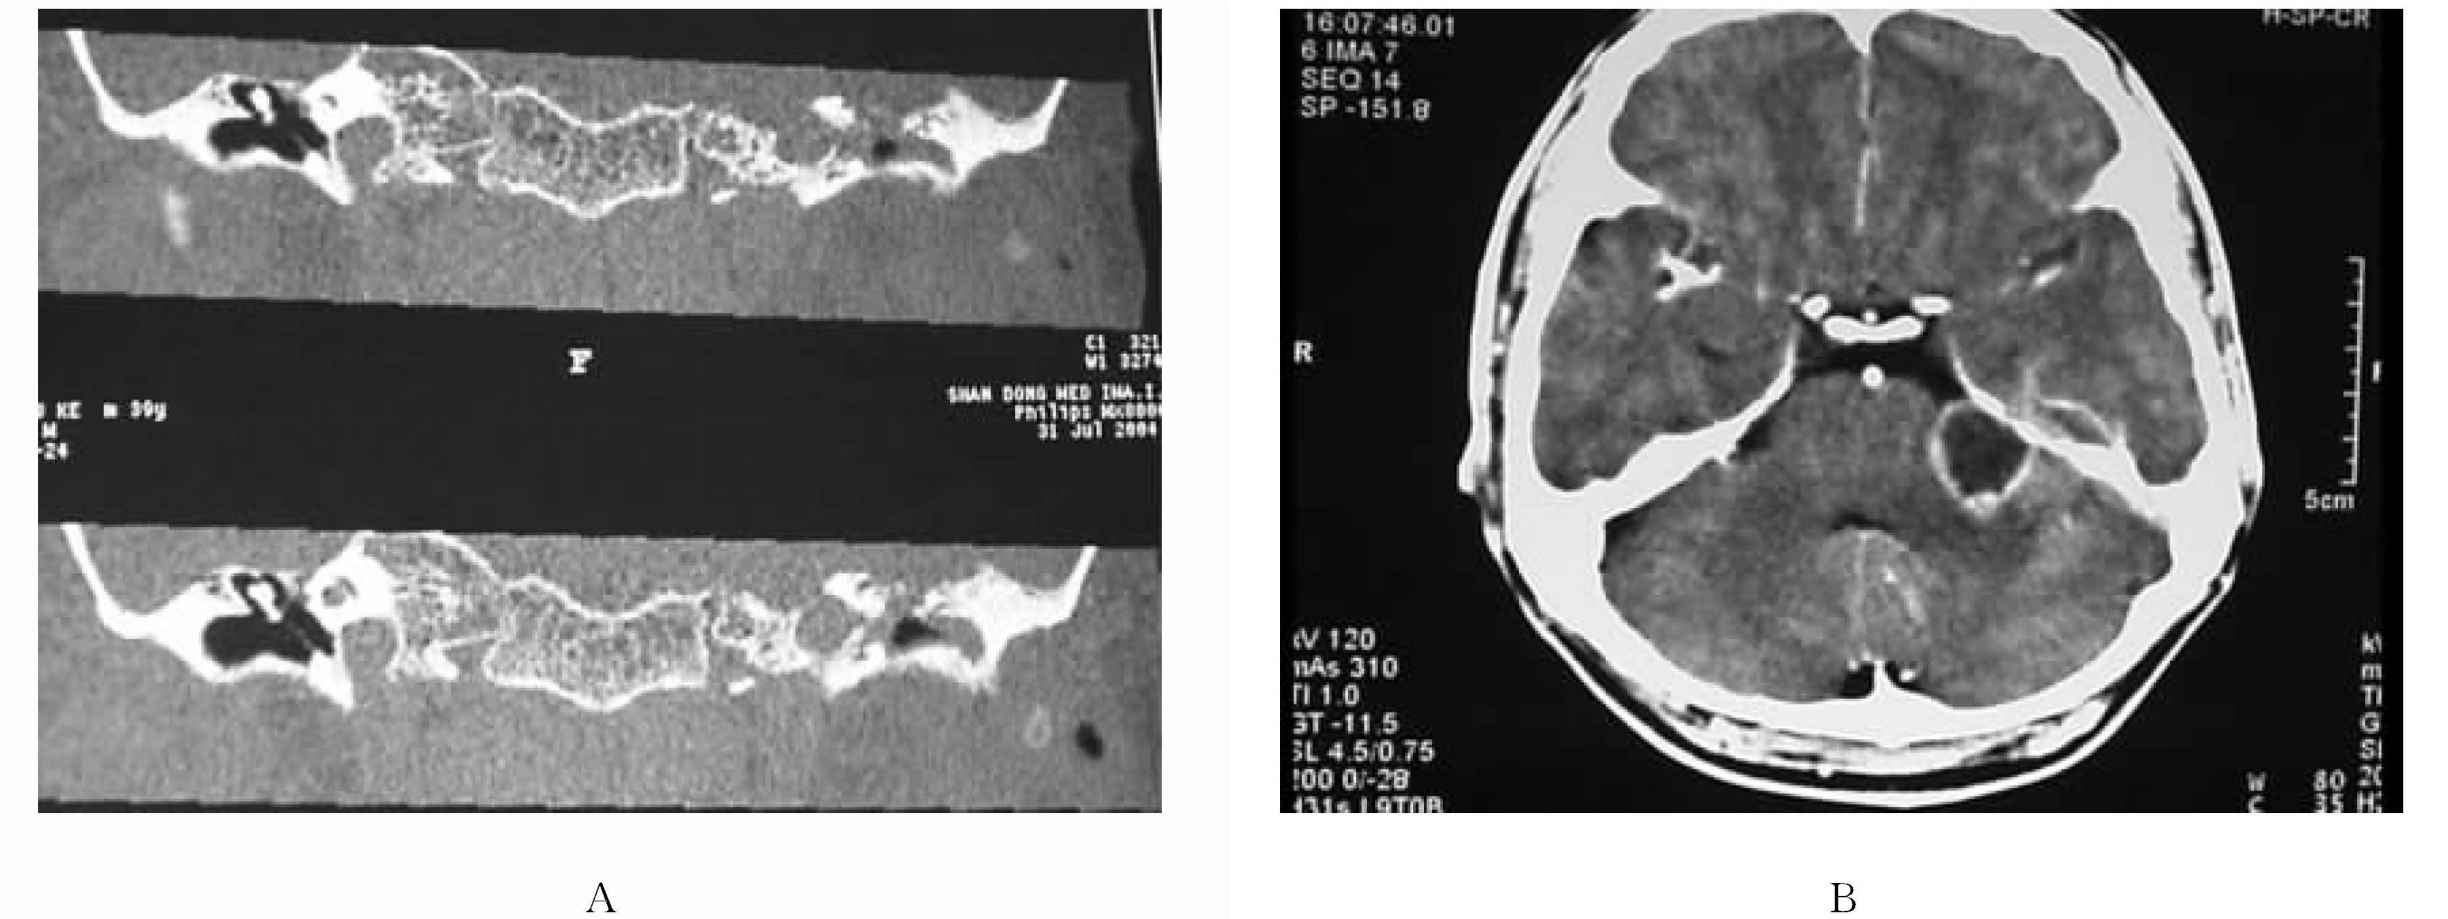
\includegraphics[width=.7\textwidth,height=\textheight,keepaspectratio]{./images/Image00121.jpg}
 \captionsetup{justification=centering}
 \caption{左侧中耳乳突炎并左侧小脑脑脓肿}
 \label{fig4-5}
  \end{figure} 

\subsection{颞骨部胆固醇肉芽肿}

胆固醇肉芽肿又称胆固醇囊肿、巧克力囊肿。在头面部好发于中耳乳突,少见于鼻旁窦,为出血部位析出的胆固醇结晶引起异物反应形成的肉芽肿病变,是一种肉芽组织增生,属炎性肿块。耳镜所见似血管球瘤。

\textbf{【病理】}
炎块内含棕色半液态物质,有亚急性和慢性出血,液态物中含胆固醇,有多数巨噬细胞胞浆内有含铁血黄素和无定型的角质素碎屑,有淋巴细胞、浆细胞、嗜酸细胞、异物巨细胞浸润。

\textbf{【CT表现】}
好发于上鼓室及鼓窦入口,较少发生于岩部。可显示无强化的软组织肿块,骨质破坏较轻微。但发生于岩尖者可有类似胆脂瘤的破坏。

\textbf{【鉴别诊断】}
主要与胆脂瘤鉴别:①本病与胆脂瘤病理有别,胆脂瘤由鳞状上皮构成,亦含脱落的角质素碎屑、出血及胆固醇结晶,但不含肉芽组织及细胞浸润;②本病CT所见不能与胆脂瘤区分;③MR检查胆固醇肉芽肿于T\textsubscript{1}
及T\textsubscript{2} 加权均呈高信号,而胆脂瘤T\textsubscript{1}
加权为中等信号,T\textsubscript{2} 加权像为次高信号可予鉴别。

\subsection{结核性乳突炎}

本病多由体内结核灶经血行或咽喉部结核菌直接经咽鼓管进入鼓室而发病。

\textbf{【病理】}
结核杆菌先感染黏膜,后及骨膜,最后侵入骨髓。其病理改变可分为粟粒型、肉芽型和干酪型。

\textbf{【临床表现】}
常见于5~6岁儿童,成人很少见。无急性病史,常有耳道流出稀薄脓液及听力减退。早期出现合并症,其中以耳后脓肿最多见,瘘管常见,少数可出现面瘫。

\textbf{【CT表现】}
中耳腔内有肉芽和渗液而密度增高,听小骨多破坏消失。乳突骨质疏松,可见弥漫性或局限性骨质破坏。局限性破坏边缘无硬化,且不规则,与正常骨质无明显分界,破坏区有细小死骨片。有文献认为耳蜗瘘是结核的特征性表现。

\textbf{【鉴别诊断】}
本病与非结核性炎症有相似改变,结合临床表现和骨破坏区内有死骨可以区别。其与胆脂瘤的膨胀性改变不难鉴别。恶性肿瘤骨破坏区中无明显死骨,破坏内耳结构也少见,结合临床也可鉴别。

\subsection{骨化性迷路炎}

本病又称为硬化性迷路炎、钙化性迷路炎和闭塞性迷路炎。在正常透明的耳蜗及前庭管腔内有新生骨充填,是内耳各种非肿瘤性病变的转归。

\textbf{【病因病理】}
本病的主要病因是脑膜炎(包括病毒性、细菌性)。最常见的是病毒感染,其次细菌感染多继发于中耳炎或脑膜炎,而梅毒性及自体免疫性迷路炎少见。90%以上发生于膜迷路炎症后几个月。少见的病因为耳硬化症、外伤、耳毒性药物治疗及特发渐进性感音聋。以上各种疾病均可导致膜迷路的感觉性神经上皮丧失造成听力损失,同时疾病的慢性刺激引起迷路内纤维组织形成,最终导致骨化。

\textbf{【临床表现】}
本病比较少见。患者可重度感音性耳聋,部分可有脑膜炎、化脓性中耳炎、高热等病史,其他无明确病史。

\textbf{【CT表现】}
HRCT可见内耳迷路不同程度、不同范围的密度增高,并可清晰显示内耳迷路内不同程度的骨化。文献报道其诊断准确率为53%~75%,原因为早期纤维化、高分辨成像密度分辨率低以及部分容积效应,不能显示早期的少量钙化骨化。此外,炎性迷路炎早期的典型影像学表现为MR
T\textsubscript{1} WI增强扫描呈明显强化。

\textbf{【鉴别诊断】}
①内耳膜迷路全部骨化需与耳蜗未发育鉴别,主要根据听囊径的大小。先天畸形患者听囊径均减小,而骨化性迷路炎的患者正常。②Michel畸形内耳外侧壁扁平,而骨化性迷路炎外侧半规管的轮廓正常。

\subsection{耳硬化症}

本病又称为耳海绵化症。迷路正常骨质被疏松海绵状骨所代替,并可硬化增生。本病多为双侧性(85%),其病因多认为系骨迷路营养障碍所致,可有遗传倾向。

\textbf{【病理】}
分为充血期、海绵化期和硬化期3期,亦可将充血期及海绵化期总称为活动期,硬化期称为静止期或成熟期。活动期骨小梁网状结构稀疏、不规则,伴随大量血管、成骨细胞、破骨细胞;成熟期病灶由相对无血管、非细胞的致密骨组成。按受累部位分为窗型及窗后型。病变可涉及听小骨、内耳迷路骨部,引起广泛骨质硬化。

\textbf{【临床表现】}
多在10~40岁发病,常见于20~30岁的女性,男女之比约1∶2,妊娠期加重。主要表现为鼓膜正常的传导性、感音性或混合性耳聋,听力减退常呈进行性,另有耳鸣、眩晕等。

\textbf{【CT表现】}
①窗型较早期示前庭窗缘骨质吸收,前庭窗“扩大”。较晚期可显示蹬骨底板增厚、前庭窗缘增厚,前庭窗变小或封闭,亦可累及蜗窗。②窗后型主要累及耳蜗。由于骨迷路海绵化(骨质疏松)致耳蜗密度减低,密度明显不均;连续的低密度灶似透明环状,形成典型的“双环征”;密度减低区间有小硬化灶。耳蜗与周围骨质界限模糊或中断。硬化期表现为活动期的骨质松化逐渐修复硬化,密度增高,骨质增厚。

\textbf{【鉴别诊断】}
蹬骨耳硬化症的鉴别包括先天性蹬骨固定、听小骨异常、外伤性听骨链断裂、鼓膜硬化。耳蜗硬化症应注意与畸形性骨炎、梅毒性中耳炎、先天性成骨不全鉴别。

1.晚发性成骨不全:可见骨迷路包括前庭、耳蜗、半规管广泛骨质增厚,密度增高。与耳硬化症不同的是听小骨发育小,常见蹬骨脚骨折,不能与底板连接。此外尚可见中耳黏膜增生、出血、鼓室狭窄。骨质病变较耳硬化症广泛,并累及鼓室。蹬骨全部、部分患者面神经鼓室段被包埋于增生的骨质内。

2.鼓室硬化症:与耳硬化症非同一概念。本病为鼓室内玻璃样变物质沉着或肉芽组织纤维化、钙化。可见于鼓膜、听小骨、鼓岬、上鼓室,不涉及内耳。

\section{肿瘤和肿瘤样病变}

\subsection{外耳道及乳突肿瘤}

\subsubsection{骨瘤}

多为致密骨瘤,颞部骨瘤常发生于外耳道或乳突近窦硬膜三角区。

\textbf{【CT表现】}
①外耳道骨瘤:多位于外耳道开口处。表现为类圆形光滑致密骨块,如阻塞外耳道可发生外耳道炎,甚至中耳乳突炎。②乳突骨瘤:多表现为乳突外板致密的骨性突起,表面圆隆,界限清楚。

\subsubsection{外耳道乳头状瘤}

是耳科常见的良性肿瘤,为复层鳞状上皮的乳头状增生,与病毒感染有关。潜伏期几个月至十年之久,手术不彻底易复发,且可有恶变。

\textbf{【CT表现】}
外耳道内增强明显的软组织肿块,密度均匀或不均匀;未充满耳道者可见其表面呈乳头状。耳道无改变或膨大,骨质多无改变或轻度吸收。肿瘤大者向外涉及耳甲腔,向内涉及鼓室。如有恶变则会出现不规则骨质破坏并侵及邻近骨结构。

\subsubsection{耵聍腺瘤和耵聍腺癌}

外耳道腺细胞起源的肿瘤很少,腺细胞指汗腺、耵聍腺(一种特殊的汗腺)和皮脂腺的细胞。其中,以耵聍腺瘤常见。

\textbf{【CT表现】}
外耳道软组织肿块,如合并有溶骨性骨质破坏,应考虑为耵聍腺癌。

\subsubsection{外耳道原发恶性肿瘤}

常见的有鳞状上皮癌,其次为腺样囊性癌。鳞癌起源于外耳道鳞状上皮,也可由乳头状瘤恶变而来。

\textbf{【CT表现】}
早期可见外耳道内软组织增生,强化显著,密度不均,界限不清。进一步发展引起不规则溶骨性骨质破坏,进而广泛侵及周围组织结构和中耳,而难以区分其原发部位。可发生局部淋巴结和远处转移。

\subsubsection{转移瘤}

外耳和乳突的转移瘤少见。

\textbf{【CT表现】}
可表现为溶骨性骨质破坏和软组织肿块。但无特异性,需结合临床综合诊断。

\subsection{血管球瘤}

血管球瘤也称为化学感受器瘤、非嗜铬性副神经节瘤。起源于头、颈部几个部位的化学感受器细胞。化学感受体是由上皮细胞形成的小体,由毛细血管和少量纤维分隔成细胞巢。只有感觉神经,不嗜铬,无内分泌功能,可感受血中酸碱度、温度、O\textsubscript{2}
和CO\textsubscript{2} 张力的改变。

\textbf{【病理】}
大多为良性,主要由非嗜铬染色的嗜铬细胞所组成,少数为恶性,并可血行或淋巴转移。头颈部血管球瘤根据部位可分为:①鼓室型:位于中耳内(起源于鼓岬的舌咽神经鼓支);②颈静脉型:位于颈静脉孔内(来源于颈静脉外膜的迷走神经耳支);③迷走神经型:位于口咽和鼻咽部的颈动脉间隙内;④颈动脉体型:位于颈动脉分叉。此外,肿瘤同时累及颈静脉孔和鼓室者叫颈静脉鼓室球瘤。

\textbf{【临床表现】}
鼓室型及颈静脉鼓室型(也称为鼓室球瘤或颈静脉鼓室球瘤)的常见表现有:①搏动性耳鸣;②蓝色鼓膜;③传导性耳聋;④颅神经损害。

\textbf{【CT表现】}
①鼓室型:表现为鼓室内小的软组织肿物,有显著强化,最大强化时间晚于颈动脉,早于颈静脉,很少发生骨质破坏。②颈静脉鼓室型:除上述表现外,可见颈静脉孔区亦有与之相延续的软组织肿物及颈静脉孔扩大等表现;良性者颈静脉孔骨质受压变形和吸收,若有不规则骨质破坏则很有可能恶变。

\textbf{【鉴别诊断】}
①高位颈静脉球:临床亦有搏动性耳鸣和蓝色鼓膜,CT表现颈静脉球高位,达中下鼓室水平,有时甚至达内耳道水平,但形态正常。除了鼓室的骨质缺损外,其他部分皮质骨清楚完整,无软组织肿块。②颈静脉孔区神经源性肿瘤:强化不及颈静脉球瘤。③鼓室内血管瘤:难以鉴别。

\subsection{原发性胆脂瘤}

本病又称为真性胆脂瘤,为先天性疾病。

\textbf{【病因病理】}
原发性胆脂瘤是胚胎上皮残留在颞骨内所形成的,多数发生在岩锥,少数发生在乳突、中耳、鼓乳缝等区域。其病理改变与继发性相同,均为脱落角化上皮堆积。

\textbf{【临床表现】}
面瘫、耳聋等症状,无流脓和鼓膜穿孔等慢性中耳乳突炎的表现。

\textbf{【CT表现】}
典型表现为岩锥部圆形骨缺损腔,边缘清楚、光滑,可有骨质硬化。骨缺损腔可涉及内耳道、面神经管等区。病灶呈均匀性囊状低密度,CT值多为30~50Hu,或呈负值。其密度及CT值无特异性,增强扫描无强化。

\textbf{【鉴别诊断】}
中耳乳突无异常,且不存在继发性胆脂瘤的破坏途径(故一般无鼓膜嵴吸收破坏)是与继发性相鉴别的要点。但有时原发性与继发性可并存。

\subsection{面神经瘤}

面神经分为6段:①颅内段(又称脑池段);②内耳道段;③迷路段;④鼓室段(又称水平段);⑤垂直段(又称乳突段);⑥腮腺段(又称颅外段)。

\textbf{【病理】}
面神经瘤为良性肿瘤,多为神经鞘瘤,常发生于面神经前膝部和乳突段。神经纤维瘤少见(多发生在婴幼儿和儿童),极少数是神经纤维瘤病的一种表现。

\textbf{【临床表现】}
典型表现为缓慢渐进性面神经麻痹,亦可突然发作或间歇发作,并出现半面痉挛。第二个常见表现是听力下降(感音性、传导性或混合性)。此外,还可表现为耳鸣、耳痛和眩晕等症状。

\textbf{【CT表现】}
①迷路段、膝部、鼓室段和垂直段面神经瘤:表现为面神经管扩大和(或)骨质破坏,以及强化的软组织肿块。国外有学者认为面神经瘤呈延迟强化,并有学者认为膝状窝处骨质膨胀性改变是其特征。鼓室内软组织肿块可压迫听小骨使之移位或破坏。②内听道段面神经瘤:表现为内听道软组织肿块,可破坏内听道前上方骨质。并可向前破坏迷路段和膝神经窝骨质突入中颅窝,向内通过内耳门突入桥小脑角而形成该区肿块。这在CT上形成典型的由内听道与面神经管沟通的桥小脑角区和中颅窝面神经瘤,此征象是与听神经瘤相鉴别的特征性征象。否则如面神经瘤局限于内听道或桥小脑角区则与听神经瘤难以鉴别,但如肿瘤偏于内听道长轴前上方生长,则高度提示为面神经瘤。

CT诊断的局限性:①桥小脑角区和中颅窝肿块及腮腺内面神经瘤CT显示较差,易漏诊。②CT上显示颞骨内软组织影的真实度和有无强化效果较差。与鼓室内或乳突内的其他肿块鉴别困难。③CT诊断内听道内小面神经瘤较困难。④胆脂瘤或胆固醇肉芽肿也表现为骨质破坏和软组织肿块,无强化有助于鉴别,但有时鉴别困难。

\subsection{耳血管瘤}

本病少见,可发生于外耳道、鼓室、鳞部或岩部。

\textbf{【临床表现】}
早期症状是搏动性耳鸣和听力下降,以后有面瘫及耳道出血等症状。

\textbf{【CT表现】}
①外耳道或鼓室内边缘模糊的软组织肿块,可侵蚀听小骨,但不破坏鼓室底。②颞骨部血管瘤呈密度不均的骨质破坏区,边缘不规整,典型者呈辐射状或针状结构,有膨胀性。③岩尖部者可呈蜂窝状结构,其内充以软组织,并有膨胀性,边缘不整。

\textbf{【鉴别诊断】}
鼓室内血管瘤与鼓室球瘤(即血管球瘤)影像表现相似,难以鉴别。如有鼓室下壁破坏,则以鼓室球瘤或颈静脉球瘤可能性大。

\subsection{中耳癌}

本病为临床较常见的恶性肿瘤,远较外耳癌多见。

\textbf{【病因病理】}
约75%继发于化脓性中耳乳突炎,故长期慢性炎症可能为其病因。绝大多数为鳞状细胞癌,其他类型少见。

\textbf{【临床表现】}
多见中老年人。除长期慢性化脓性中耳乳突炎的表现外,还有耳道流血性分泌物、疼痛、面瘫等。

\textbf{【CT表现】}
鼓室内软组织肿物及骨质破坏,边缘不规整。骨质破坏发展方向不一,听小骨不规则破坏。增强后多明显强化,亦可强化不显著。病变发展表现为以鼓室为中心的弥漫性软组织增生和虫蚀样骨质破坏。

\textbf{【鉴别诊断】}
中耳癌密度高,强化明显,骨质破坏呈不规则虫蚀状,听小骨破坏完全,鼓室各壁均吸收破坏,不像慢性中耳乳突炎主要以上鼓室吸收扩大。但早期中耳癌骨质破坏不明显,可难与炎症鉴别。此外,中耳癌有耳道流血、新生物易出血表现有利于鉴别。

\subsection{颞骨横纹肌肉瘤}

本病多见于10岁以下儿童,临床可见局部隆起及外耳道肿物、疼痛等。

\textbf{【CT表现】}
颞骨广泛骨质破坏,边缘不规整。增强后肿瘤有明显强化,多超出颞骨范围。与炎症鉴别靠活检,癌多见于成人,骨质破坏区可不强化。

\subsection{颞骨组织细胞增生症}

组织细胞增生症为少见且原因不明的疾病。

\textbf{【病理】}
组织细胞异常增生是其病理特征,常见为嗜酸性肉芽肿。头颅为好发区,耳部好发于外耳道和颞鳞部。

\textbf{【临床表现】}
多见于儿童,耳部疼痛、听力下降和耳漏为常见症状,可见耳后隆起及外耳道肿块。涉及眼眶有眼球突出,涉及蝶鞍可产生尿崩症。

\textbf{【CT表现】}
颞骨乳突部或鳞部溶骨性破坏,蜂房充以软组织。鼓室和外耳道内亦可充以软组织影,外耳道骨壁破坏。软组织病灶可显著强化。骨质破坏腔边缘毛糙,无膨胀性,与恶性肿瘤难以鉴别。有的骨破坏边缘有硬化,多发破坏灶呈地图样有助于诊断。

\subsection{骨纤维异常增殖症}

本病是一种生长发育障碍性疾病。

\textbf{【病理】}
骨内异常纤维组织和类骨样组织的广泛增生导致骨体积增大。病变组织内无成骨细胞和板层样骨小梁为其特点。

\textbf{【临床表现】}
病人颞部逐渐隆起,无明显不适。外耳道可狭小或闭锁,甚至继发中耳乳突炎。

\textbf{【CT表现】}
一般为单侧性。颞骨增大增厚变形,密度不均,结构紊乱,其中有半透明磨玻璃样密度区。乳突蜂房被占据消失,鼓室变窄、变形,耳结构受压移位,含气腔狭窄变形。

\protect\hypertarget{text00012.html}{}{}

